\chapter{Creating a Proof of Concept Use for ScienceIE data}
\section{Concept and Specification}
Having completed systems to handle the information extraction, the next major part of the project was to explore how this information can be utilised for researchers. 

The most obvious domain for using summary information about a set of resources is search. Being able to efficiently search through a large set of documents to quickly find more useful information is a very useful thing. The focus of this section is to explore using the key phrase information in an efficient and convenient way to aid in user query across the ScienceIE data set. 

The ScienceIE data set is specifically being used because that is what the algorithms in this project are designed for. The problem of handling longer, full publications has been discussed, so to not complicate this investigation further, the standard short documents of ScienceIE shall form the database of documents.

The following requirements are presented for the POC system to conform to are:
\begin{enumerate}
	\item As a basis to make the system usable, the ability to list papers in the database, and the ability to present all the information about a paper on one screen. The ability to download the extractions in the BRAT format should also be made available. 
	\item A search system for the key phrase information gained. This should allow the input of a user query (plain natural language text), with an option to give some indication of the classification of the information they are interested in (i.e. \textit{task}, \textit{process} or \textit{material}).
	\item The ability to add papers dynamically to the database throughout run time. This means not only should the system support the creation of new paper records, but also the automatic processing of that paper through all 3 subtasks of ScienceIE, with the results being available to the search system.
	\item Some way of conveying summary information about the extractions contained in the system. While not essential for search, having a convenient way for the developer and users to take a snapshot of what is contained in the system is useful for evaluation purposes, including giving an indication of how many papers are included and their processing status.
\end{enumerate}

\section{Background and Technology Review}
\subsubsection*{Existing Search}
Two popular, publicly available search engines have been examined to extra some well designed features from. These are Google Scholar\footnote{\href{https://scholar.google.com/}{https://scholar.google.com/}} and ScienceDirect\footnote{\href{https://www.sciencedirect.com/}{https://www.sciencedirect.com/}}, and appendix \ref{appendix:searcheg} shows screen shots of both web sites given the same query. Common features are:
\begin{itemize}
	\item Limited results per page (10 on Google Scholar, 25 on ScienceDirect),
	\item The total number of documents selected and the time it took to do this is displayed to the user,
	\item Filtering options, including by date,
	\item The title of a result is followed by a snippet of the document, with relevant words highlighted in some way,
	\item The title is a link to an individual results page which presents information about the document, but there are also links to directly get the document downloaded.
\end{itemize}

\noindent Some custom features on each website are:
\begin{itemize}
	\item ScienceDirect supports searches with multiple parameters, including query fields specifically for author, title, pages, etc...
	\item ScienceDirect also supports custom numbers of search results per page; 25 is the default, but the user can receive 50 or 100 results per page if they wish,
	\item Google Scholar present \textit{related searches} to allow the user to navigate sideways towards their target paper, rather than straight down to it,
	\item ScienceDirect features a \textit{recommended} section at the top where it showcases several publications it believes to be the most relevant.
\end{itemize}

Given the data set available in this project, most of these ideas presented by Google Scholar and ScienceDirect can be implemented. However, as ScienceIE's data is purely text snippets of documents, author, real title, publish information and more are unavailable, meaning any system created here cannot support filtering by these features, or display that information. An original hope of the developer was to include a more advanced search, potentially including a PageRank type system \cite{Page1998} where the links would be based on referencing, but unfortunately without even the reference information for each paper available, this is impossible to achieve whit the ScienceIE dataset.

The search on these two websites is likely be based on latent semantic analysis (\cite{Landauer1998} and \cite{AswaniKumar2012}) which looks at the similarities between search terms and attempts to take into account context. This method of representing words in a vector space prepared for querying is a popular method of document retrieval. This method of querying could potentially be modified to involved more weighting of tokens if the are included in key phrases, or be used to inspire a new algorithm that uses key phrase information to help with weighting word importance.

\subsubsection*{Available Technologies}
The goal with this project is to prove a use of the data produced as part of ScienceIE through some application. To make this application available for use, a web based service will be created that allows any user to join without the need for complex setup. The benefits of this include not having to distribute installation media and update media, along with centralised management of any database of information and being able to immediately make available new features.

In terms of storing information, popular database technologies were surveyed. The stack overflow survey 2017 listed MySQL\footnote{\href{https://www.mysql.com/}{https://www.mysql.com/}} as the most used SQL platform by developers on the sight\footnote{\href{https://insights.stackoverflow.com/survey/2017\#technology-databases}{https://insights.stackoverflow.com/survey/2017\#technology-databases}}. One reason for this is that some competitive SQL platforms require licensing (especially when commercial use is considered), such as Oracle SQL, while MySQL is open source and can be used more freely. The platform can be easily acquired and installed on various platforms (with major Windows and Linux operating systems supported), with largely straight forward initial configuration (for a project of this scale). The standard MySQL installation also includes the MySQL Workbench, which includes a convenient tool for building a relational database schema\footnote{\href{https://dev.mysql.com/doc/workbench/en/wb-data-modeling.html}{https://dev.mysql.com/doc/workbench/en/wb-data-modeling.html}}, with the ability to export SQL scripts to build the designed database in a single execution (including tables, relations and users with certain access rights). 

One of the most popular Java web frameworks available is Spring. Spring provides functionality to route requests to certain Java classes for processing, including the passing of any parameters with some degree of automatic validation, and the ability to process Java Servlet Pages (JSPs) which are compiled at run time to delivery varying pieces of information to the end users. It implemented the standard \textit{model-view-controller} (MVC) design pattern. To keep the focus on the use of data processed in this project, a convenient web container is desired, and that is what Spring Boot\footnote{\href{https://projects.spring.io/spring-boot/}{https://projects.spring.io/spring-boot/}} provides. This packages the Spring technology stack, web server technology (for example, Apache Tomcat) and any extra libraries required into a single, executable, Java project, making heavy use of annotations for the minimal configuration required. This makes it an extremely portable and (in terms of environment and system configuration) light weight application to set-up and run, which reflects as part of their projects mission statement to get developers "up and running as quickly as possible". It is a young project, with the original version being released in 2014 and version 2.0 being released during the course of this project, meaning it is built to work with the current standard of industrial Java technologies - so while this project is aiming to build a simple application, it shall have some powerful technologies standing behind it.

% TODO find a reference for MVC?

One of these technologies is Hibernate\footnote{\href{http://hibernate.org/}{http://hibernate.org/}}. This integrates with the Java Persistance API (JPA), supported by Spring, for extremely simply database interactions with many functions being supported by default. It combines a simple Java object which holds fields relating to each of the column in a database entity (table), and an abstract \texttt{CrudRepository} class which can be extended from to make a data access object which can retrieve records from a database and update them as well. Methods can be added to the extended class to make more complex queries, and either plain English can be used in the method name to define the query, or the specific SQL query statement can be specified if required\footnote{A guide to using this technology is freely available on Spring's website and is presented in a very simple manor. It can be viewed at \href{https://spring.io/guides/gs/accessing-data-jpa/}{https://spring.io/guides/gs/accessing-data-jpa/}} Furthermore, when fields are foreign keys of other entities, rather than being of an \textit{ID} type such as \texttt{Integer} or \texttt{Long}, the class representation of the foreign entity can be used instead, and Hibernate will automatically populate it with the correct object.

\section{Design and Configuration}

\subsection*{Design of the Services}
There are four key requirements of the POC system which cover a large amount of usability. The first requirement is very simple. Two pages are required for this:
\begin{itemize}
	\item The first is simply a list of papers, each selectable. When selected, the user will be taken to the next paper described.
	\item The second page, for displaying information about a paper, should begin with the title at the top, a section in the middle for the original text, and finish with a list of key phrases and relations. The key phrases, as a minimum, should be annotated on the main text as well.
\end{itemize}

The second requirement is covering the question of search. A new algorithm is proposed that includes the key phrase information about a paper. Using the concept of using the TF-IDF scores of both the tokens in all documents as well as the tokens in the query to try to find papers is utilised with a scaling factor, defined by the presence of key words in a paper.

\subsection*{Database Design and Entity Relationship Diagram}

\begin{figure}
	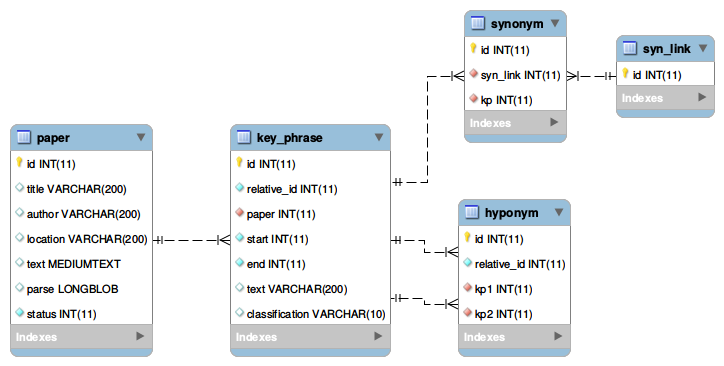
\includegraphics[width=\textwidth]{img/fypdberd.png}
	\caption[Database Entity Relationship Diagram]{The entity relationship diagram that supports this proof-of-concept system, as exported from the MySQL Workbench tool kit. Primary keys are represented by gold keys, foreign keys are red diamonds, normal fields are blue diamonds and hollow blue diamonds indicate the field is nullable. Types for all fields in all entities are also shown. The Java representation of these entities share the same name in all cases, converted to camel case, aside from the entity titles which have \texttt{DAO} appended (standing for \textit{data access object}) as without this the class names would clash with those used in the NLP system, which would have been confusing to program with. As examples, the \texttt{paper} entity was \texttt{PaperDAO} in the Java project, but an \texttt{id} field would remain \texttt{id} in the Java code to follow the standard.}
	\label{figure:dberd}
\end{figure}

The support storage and query of the data produced by the ScienceIE task, a suitable database must be designed and created. Given a lot of the required entities had been created as part of the NLP system, the data base design heavily inherits the classes and fields from this. The full design for the database is shown in figure \ref{figure:dberd}

The \texttt{paper} and \texttt{key\_phrase} entities are largely the same as their equivalents in the NLP system. Of course, rather than having a list of key phrases held within the \texttt{paper} entity, the \texttt{key\_phrase} entity has a field to store a reference to its parent \texttt{paper}. The \texttt{paper} entity also has two fields no in the NLP system: a \texttt{status} which was discussed above, and a \texttt{parse} which holds a serialised \texttt{Paper} Java object. This allows the preprocessing to take place and for that information to be stored directly in the database with its parent record, removing the need for re-computation of preprocessing every time the paper is called from the database.

The method for storing hyponyms and synonyms is slightly different to the NLP system. Rather than being part of a relations list the parent paper record holds, instead each relation holds the \texttt{key\_phrase} references they are a relation of. The original \texttt{paper} can still be retrieved through retrieving the referenced \texttt{key\_phrase} records. The \texttt{hyponym} record holds the two \texttt{key\_phrase} records it is a relation of, as well as a relative ID, which is the ID of the hyponym relation relative to the individual paper it is from. The \texttt{synonym} relation is a little more complex. While the NLP system created didn't support more than two way synonym relation extraction and there was only one example of a three way synonym relation in the ScienceIE data set, to support the range of relations defined as part of ScienceIE these synonym entity has to support one synonym referencing a variable amount of \texttt{key\_phrase} records. Therefore, to avoid a many-to-many relation between entities, each \texttt{synonym} record holds a reference to a \texttt{syn\_link}, the concept being a set of synonyms, each referencing one \texttt{key\_phrase}, all reference the same \texttt{syn\_link} record, which makes the synonym relation between the set of referenced key phrases. Having \texttt{syn\_link} also provides a convenient way to count he number of synonyms in the system.

\section{Implementation}

\subsection*{Project Configuration}
The creation of the project involved including various dependencies in the \texttt{pom.xml} file and setting up the launch configuration for Spring Boot.

To include Spring Boot, \texttt{pom.xml} was configured as described on the Spring Boot website, along with a connector package for MySQL\footnote{\href{https://spring.io/guides/gs/accessing-data-mysql/}{https://spring.io/guides/gs/accessing-data-mysql/}}. 

\begin{figure}
	\begin{lstlisting}[language=XML]
<dependency>
  <groupId>xyz.tomclarke.fyp</groupId>
  <artifactId>fyp-nlp</artifactId>
  <version>0.0.1-SNAPSHOT</version>
  <!-- Stop logging dependency errors -->
  <exclusions>
    <exclusion>
      <groupId>ch.qos.logback</groupId>
      <artifactId>logback-core</artifactId>
    </exclusion>
    <exclusion>
      <groupId>org.slf4j</groupId>
      <artifactId>slf4j-log4j12</artifactId>
    </exclusion>
  </exclusions>
</dependency>
	\end{lstlisting}
	\caption[Configuration to set the NLP system as a dependency in Maven]{The Maven configuration for listing the NLP project as a dependency, as used in the POC system. Note, the exclusion (as discussed) are to remove logging dependency conflicts using Spring Boot causes; this may break logging if another system uses this configuration but doesn't have its own logger available.}
	\label{figure:nlpdependency}
\end{figure}

To use the NLP system built in this project, Maven also needed to be told to import this so it can be used to generate information about given papers when the full system has been developed. Given the NLP system has been compiled and installed to the local Maven repository (as it is not hosted anywhere), the configuration shown in figure \ref{figure:nlpdependency} will include the NLP system in a compiled project. Doing this also sets any dependencies of the NLP system as dependencies of this system, so they do not need to be re-listed as dependencies. The unfortunate effect of this is where there are conflicts between dependencies, which is what happened in this project. The logging included in Spring Boot was an alternate version to that in the NLP project, and while it didn't damage any part of the system, on every boot it would choose one of the loggers and print out many error messages warning the developer against it. Therefore, the conflicting dependencies in the NLP system were excluded to remove this problem, and this was done to the NLP system rather than to Spring Boot as this problem may occur if the NLP system was used in another project including other dependencies, so it made sense to list how to fix it for the NLP system dependency. 

For the system to launch, some basic configuration had to be set. There is an \texttt{application.properties} file in the Java resources with the following parameters (with explanations as to why those were chosen appended):
\begin{itemize}
	\item \texttt{server.port=8080} 8080 is a standard port for testing web applications on. Furthermore, port 80 needs administrative privileges to be used ever time the application is launched, which would not only be frustrating to a developer, but not supporting good security standards if there was a vulnerability in the web service. The router the developer system was sitting behind, through port forwarding, allowed incoming connections on port 80 to be directed to 8080 on the developer system, so when connecting via web browser, no port would be needed to be specified.
	\item \texttt{debug=false} If \texttt{true} was set, this would output all debug information to the console. Given the log4j configuration being used output all debug information to disk, there was no need to have it also in console, making it harder to see what was going on while running.
	\item \texttt{spring.jpa.hibernate.ddl-auto=none} This parameter has several different possible values. \texttt{none} means the connection to the database is standard, allowing the Java application to commit reads and writes. Other values were possible, which would support (if the database hasn't been setup) automatic configuration of the database based on the entity declarations. While this could have been useful, control of configuring the database being left to the entity relationship software included in the MySQL workbench seemed preferable.
	\item \texttt{spring.datasource.url=\newline jdbc:mysql://tomclarke.xyz:3306/fyp?verifyServerCertificate=false\&useSSL=true} This is the JDBC connection string, allowing the system to find and connect to the database. To increase security, encryption of the connection through Secure Sockets Layer (SSL) is enabled, but as the database server is not configured with any certificate, this is set to be ignored.
	\item \texttt{spring.datasource.username=fyp\_user} This is simply the database user setup for the system to use. The permissions on this user were restricted to read and write of data in the \texttt{fyp} database, so if the application is compromised the database connection can't be used to read information from other databases on the same instance, or change the configuration of the database system. 
	\item \texttt{spring.datasource.password=$<$password$>$} This is the password of the database user for the system to login with.
\end{itemize}

Several parts of the above are concerned with, as well as required configuration, security of the database and system as whole, and while this project is not concerned with security, it is seen as good practise to include these features.

Finally, the class \texttt{FypGuiApplication} needed to be created, as it is this class that contains the classic \texttt{public static void main(String[] args)} method that starts the whole program. Along side the opportunity to include any other pieces of configuration completed through Java code, this initiated the Spring MVC technology stack.

\section{Web Interface}

\section{Testing}

\section{Conclusion}
